\documentclass[UTF8]{ctexart}
\bibliographystyle{unsrt}
\usepackage{geometry}
\geometry{a4paper,scale=0.8}
\usepackage{listings}
\usepackage{graphicx}
\title{机器学习(EE369)  Project2\\基于深度学习的生活垃圾图片分类\\Classification of Garbage Picture Based on Deep Learing}
\author{姓名:蒋逸伟 \\学号:517161910005}
\date{}
\makeindex
\begin{document}
\maketitle
\newpage
\tableofcontents
\newpage
\section{引言}
\subsection{背景介绍}
随着《上海市生活垃圾管理条例》\cite{garbage}在2019年7月1日正式开始执行,全国范围内的垃圾分类的热潮正式掀开。垃圾分类对于人类的可持续发展以及对生态环境的保护具有重要的意义,它可以帮助上游企业更好地实现资源的可回收利用以及垃圾填埋等。对于垃圾分类,传统上只能依靠人进行识别手工拣拾,耗时耗力。近年来随着深度学习技术的发展,利用搭建好的神经网络对图片进行特征提取然后进行分类识别技术已经成熟,AlexNet\cite{krizhevsky2014weird},
ResNet\cite{10.1007/978-3-319-46493-0_38}
等神经网络均在传统的CNN上进行了改进从而在CIFAR1000,ImageNet等数据集上实现了较好的分类效果,他们同样在垃圾图片分类这个任务上具有巨大的潜力。
\subsection{问题目标}
这个问题的目标在于给出一个垃圾的图片$x_i$能够将它正确的归并在\{"纸板","玻璃","金属","纸张","塑料","其他垃圾"\}中的一类。
\subsection{数据概况}
用于解决本个问题的数据集包括六类:分别包含cardboard(393), glass
(491), metal (400), paper (584), plastic (472) and trash (127).划分后的数据集:训练集:1768,验证集:328,测试集:431。

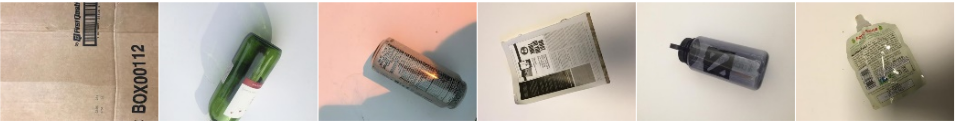
\includegraphics[scale=0.5]{gb.png}
\newpage
\section{方法与技术}
本文在上述的数据集上分别应用了AlexNet,MobileNet,DenseNet,ResNet,VGG,EfficientNet,
多种神经网络进行训练。
\subsection{AlexNet}
本深度学习网络是Alex和Hinton参加ILSVRC2012比赛的卷积网络论文,本网络结构也是开启ImageNet数据集更大,更深CNN的开山之作,本文对CNN的一些改进成为以后CNN网络通用的结构;在一些报告中被称为Alex-net,之后在Imagenet上取得更好结果的ZF-net,SPP-net,VGG等网络,都是在其基础上修改得到。\cite{NIPS2012_4824}
\begin{center}
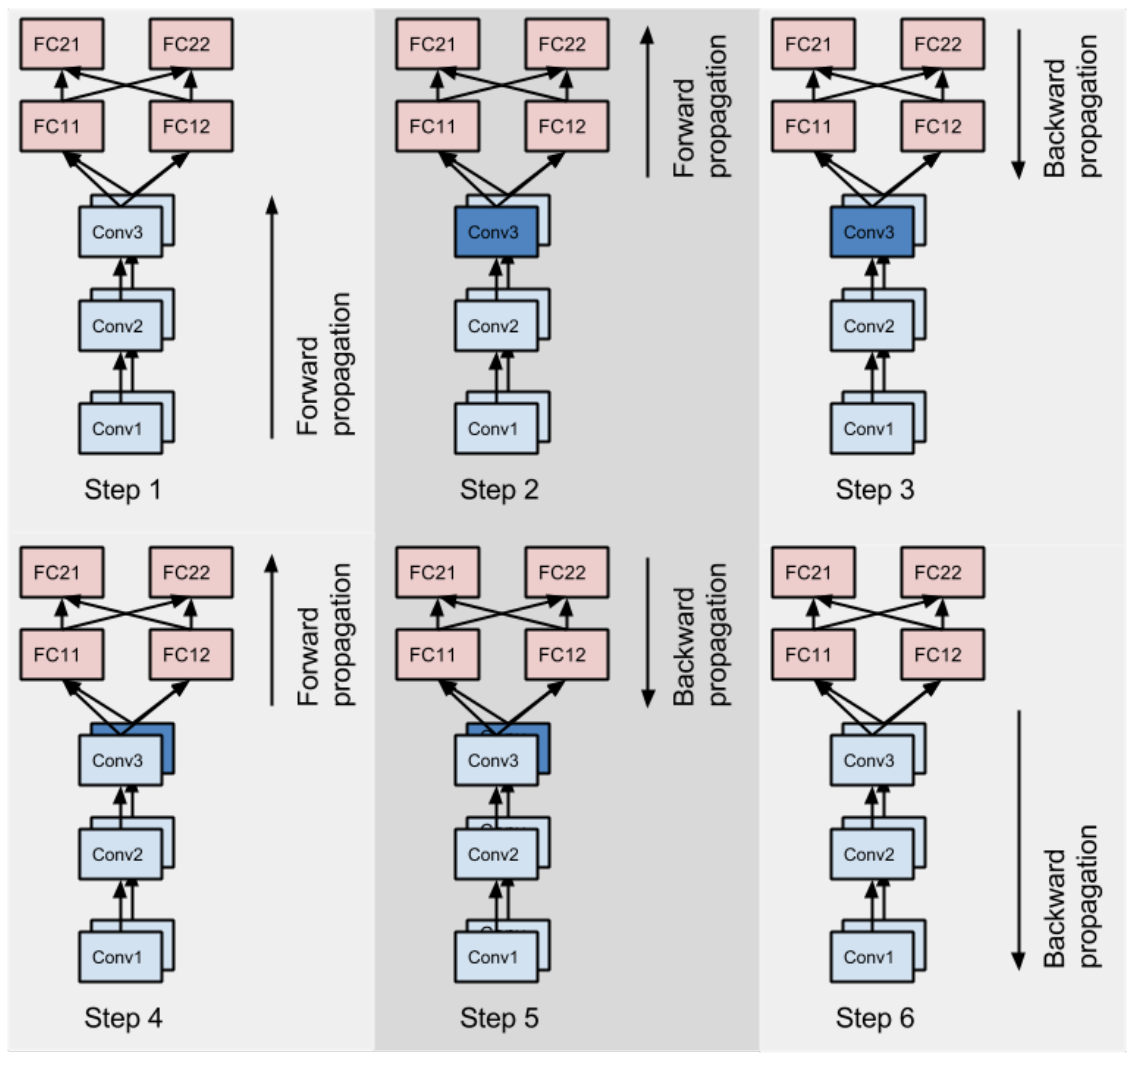
\includegraphics[height = 5cm]{alexnet.png}
\end{center}
\subsection{VGG}
AlexNet在LeNet的基础上增加了3个卷积层。但AlexNet作者对它们的卷积窗口、输出通道数和构造顺序均做了大量的调整。虽然AlexNet指明了深度卷积神经网络可以取得出色的结果,但并没有提供简单的规则以指导后来的研究者如何设计新的网络。我们将在本章的后续几节里介绍几种不同的深度网络设计思路。
它的名字来源于论文作者所在的实验室Visual Geometry Group 。\cite{simonyan2014deep}VGG提出了可以通过重复使用简单的基础块来构建深度模型的思路。
\begin{center}
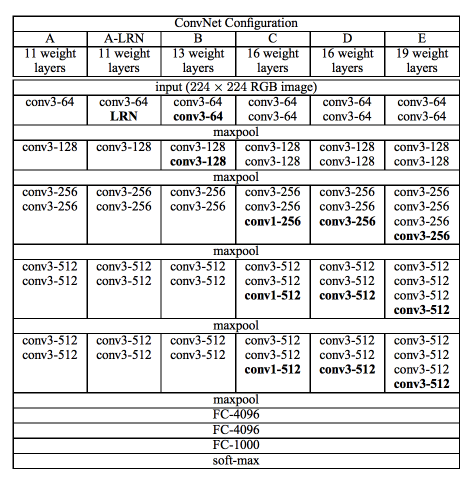
\includegraphics[scale=0.4]{vgg.png}
\end{center}
\subsection{ResNet}而Resnet\cite{10.1007/978-3-319-46493-0_38}网络作者则想到了常规计算机视觉领域常用的residual representation的概念,并进一步将它应用在了CNN模型的构建当中,于是就有了基本的residual learning的block。它通过使用多个有参层来学习输入输出之间的残差表示,而非像一般CNN网络(如Alexnet/VGG等)那样使用有参层来直接尝试学习输入、输出之间的映射。实验表明使用一般意义上的有参层来直接学习残差比直接学习输入、输出间映射要容易得多(收敛速度更快),也有效得多(可通过使用更多的层来达到更高的分类精度)。
\begin{center}
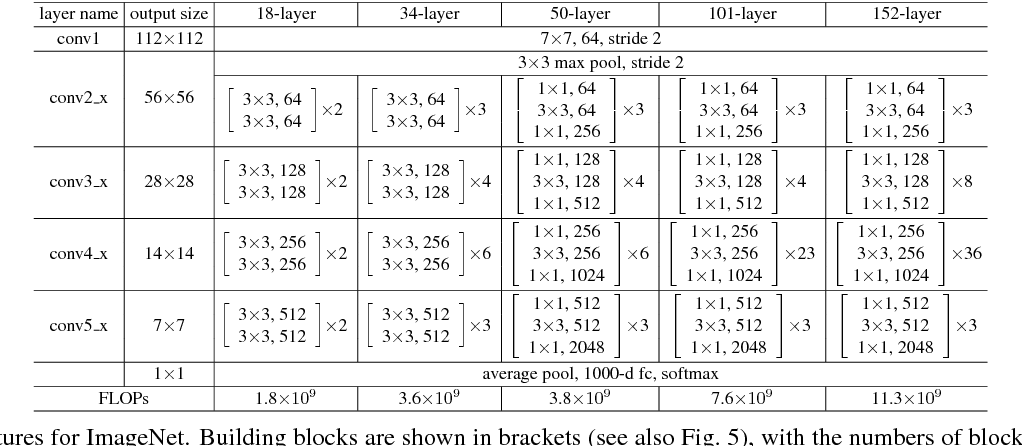
\includegraphics[scale=0.3]{resnet.png}
\end{center}
\subsection{MobileNet}
MobileNet\cite{Sandler_2018}的基本单元是深度级可分离卷积(depthwise separable convolution),其实这种结构之前已经被使用在Inception模型中。深度级可分离卷积其实是一种可分解卷积操作(factorized convolutions),其可以分解为两个更小的操作:depthwise convolution和pointwise convolution。Depthwise convolution和标准卷积不同,对于标准卷积其卷积核是用在所有的输入通道上(input channels),而depthwise convolution针对每个输入通道采用不同的卷积核,就是说一个卷积核对应一个输入通道,所以说depthwise convolution是depth级别的操作。而pointwise convolution其实就是普通的卷积,只不过其采用1x1的卷积核。对于depthwise separable convolution,其首先是采用depthwise convolution对不同输入通道分别进行卷积,然后采用pointwise convolution将上面的输出再进行结合,这样其实整体效果和一个标准卷积是差不多的,但是会大大减少计算量和模型参数量。
\begin{center}
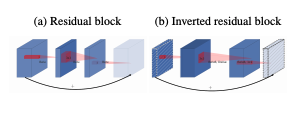
\includegraphics[scale=0.5]{mobilenet_v2_1.png}
\end{center}
\subsection{DenseNet}
\begin{center}
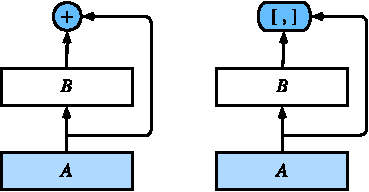
\includegraphics[scale=1]{densenet.pdf}
\end{center}

与ResNet的主要区别在于,DenseNet里模块B的输出不是像ResNet那样和模块A的输出相加,而是在通道维上连结。这样模块A的输出可以直接传入模块B后面的层。在这个设计里,模块A直接跟模块B
后面的所有层连接在了一起。这也是它被称为“稠密连接”的原因。
\subsection{EfficientNet}
\cite{tan2019efficientnet}
作者希望找到一个可以同时兼顾速度与精度的模型放缩方法,为此,作者重新审视了前人提出的模型放缩的几个维度:网络深度、网络宽度、图像分辨率,前人的文章多是放大其中的一个维度以达到更高的准确率,比如 ResNet-18 到 ResNet-152 是通过增加网络深度的方法来提高准确率。
\begin{center}
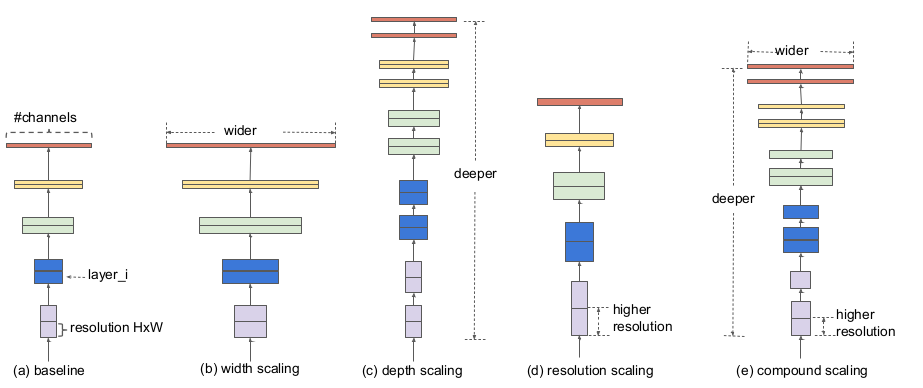
\includegraphics[scale=0.4]{efnet.png}
\end{center}
\newpage
\section{实验结果}
\subsection{未进行迁移学习(未加载与训练参数)的神经网络训练结果}
\subsubsection{AlexNet}
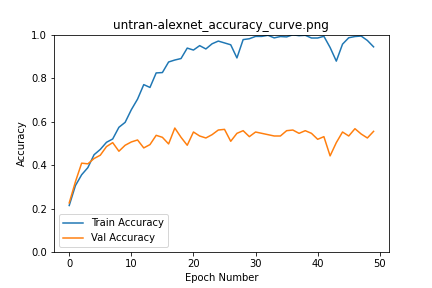
\includegraphics[scale=0.5]{image/untran-alexnet_accuracy_curve.png} 
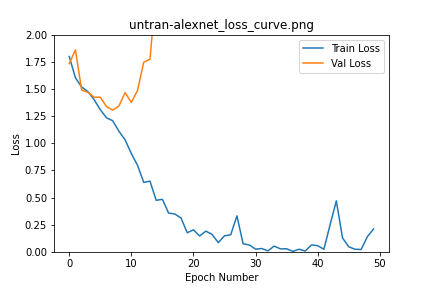
\includegraphics[scale=0.5]{image/untran-alexnet_loss_curve.png} 

在测试集上的训练结果

\begin{tabular}{|c|c|c|c|c|c|c|}
\hline 
类别 & Cardboard & Glass & Metal & Paper & Plastic & Trash \\ 
\hline 
Accuracy &0.9025522 & 0.81902552 &0.81438515 &0.77262181& 0.84686775 &0.9350348 \\
 \hline 
Recall &0.72857143& 0.48780488& 0.41176471 &0.7037037 & 0.47297297 &0.17241379 \\ 
\hline 
Precision &0.68918919& 0.52631579& 0.41176471& 0.53521127 &0.56451613& 0.55555556 \\ 
\hline 
F1 Score &0.70833333& 0.50632911& 0.41176471& 0.608      &0.51470588 &0.26315789 \\ 
\hline 
\end{tabular} 

混淆矩阵:

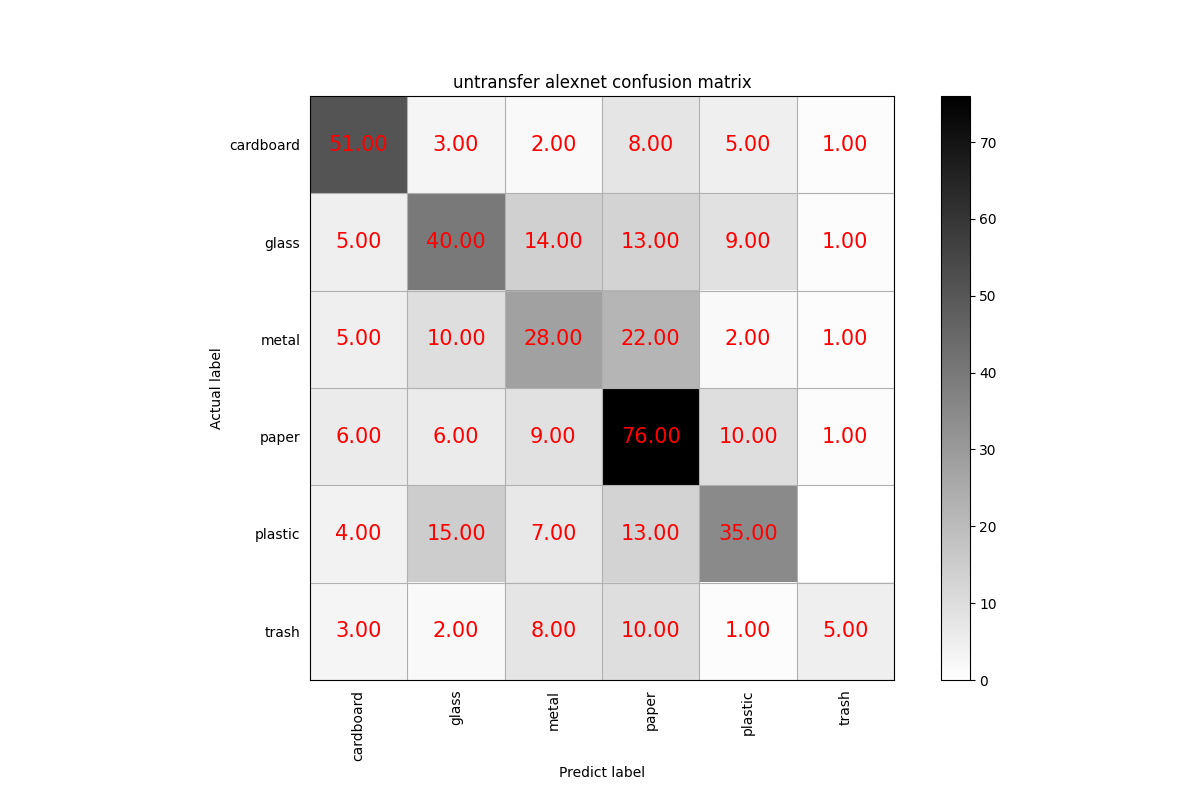
\includegraphics[scale=0.5]{cm/unalexnet.png} 
\subsubsection{VGG16\_bn}
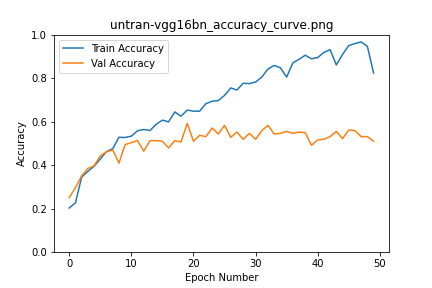
\includegraphics[scale=0.5]{image/untran-vgg16bn_accuracy_curve.png} 
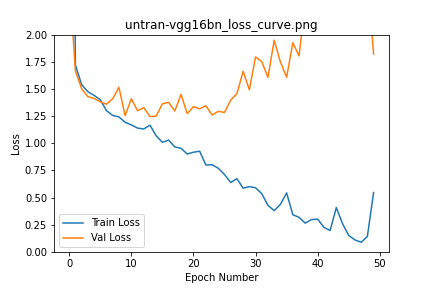
\includegraphics[scale=0.5]{image/untran-vgg16bn_loss_curve.png} 

测试集上的结果:

\begin{tabular}{|c|c|c|c|c|c|c|}
\hline 
类别 & Cardboard & Glass & Metal & Paper & Plastic & Trash \\ 
\hline 
Accuracy &0.90487239 &0.76334107& 0.87238979& 0.81670534 &0.80278422& 0.92111369\\
 \hline 
Recall &0.55714286 &0.48780488& 0.44117647 &0.57407407& 0.68918919 &0.37931034\\ 
\hline 
Precision &0.79591837& 0.4       & 0.63829787& 0.65263158& 0.45132743 &0.40740741 \\ 
\hline 
F1 Score &0.65546218& 0.43956044 &0.52173913& 0.61083744& 0.54545455& 0.39285714 \\ 
\hline 
\end{tabular}

混淆矩阵:

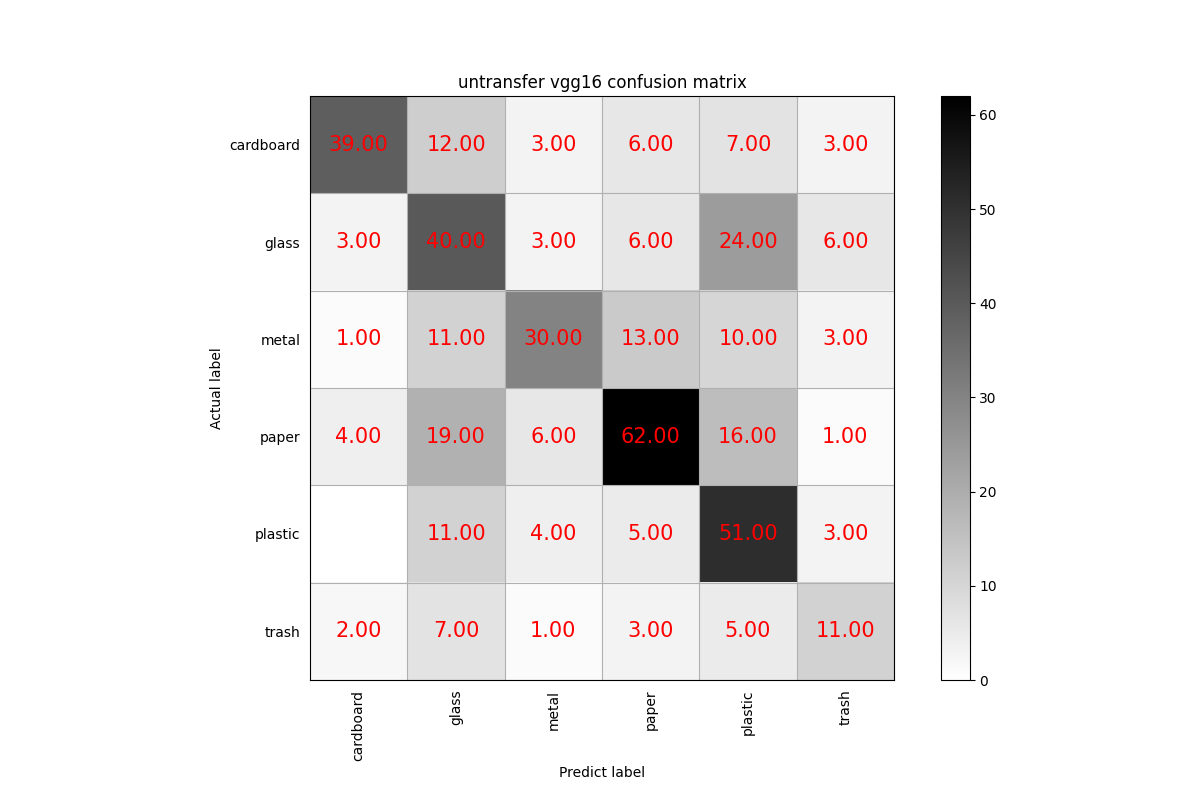
\includegraphics[scale=0.5]{cm/unvgg16.png} 
\subsubsection{VGG19\_bn}

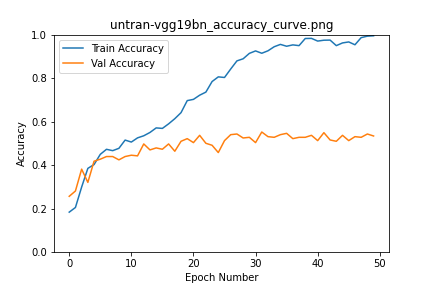
\includegraphics[scale=0.5]{image/untran-vgg19bn_accuracy_curve.png} 
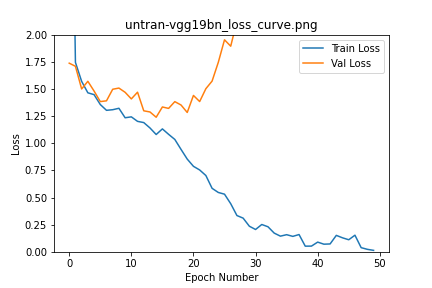
\includegraphics[scale=0.5]{image/untran-vgg19bn_loss_curve.png} 

测试集上的训练结果

\begin{tabular}{|c|c|c|c|c|c|c|}
\hline 
类别 & Cardboard & Glass & Metal & Paper & Plastic & Trash \\ 
\hline 
Accuracy &0.91183295& 0.80974478& 0.83294664& 0.83990719 &0.85382831& 0.94431555\\
 \hline 
Recall &0.72857143& 0.53658537& 0.55882353& 0.68518519& 0.47297297& 0.51724138\\ 
\hline 
Precision &0.72857143& 0.5       & 0.475   &   0.67889908& 0.59322034& 0.6   \\ 
\hline 
F1 Score &0.72857143& 0.51764706 &0.51351351& 0.68202765& 0.52631579& 0.55555556 \\ 
\hline 
\end{tabular}

混淆矩阵:

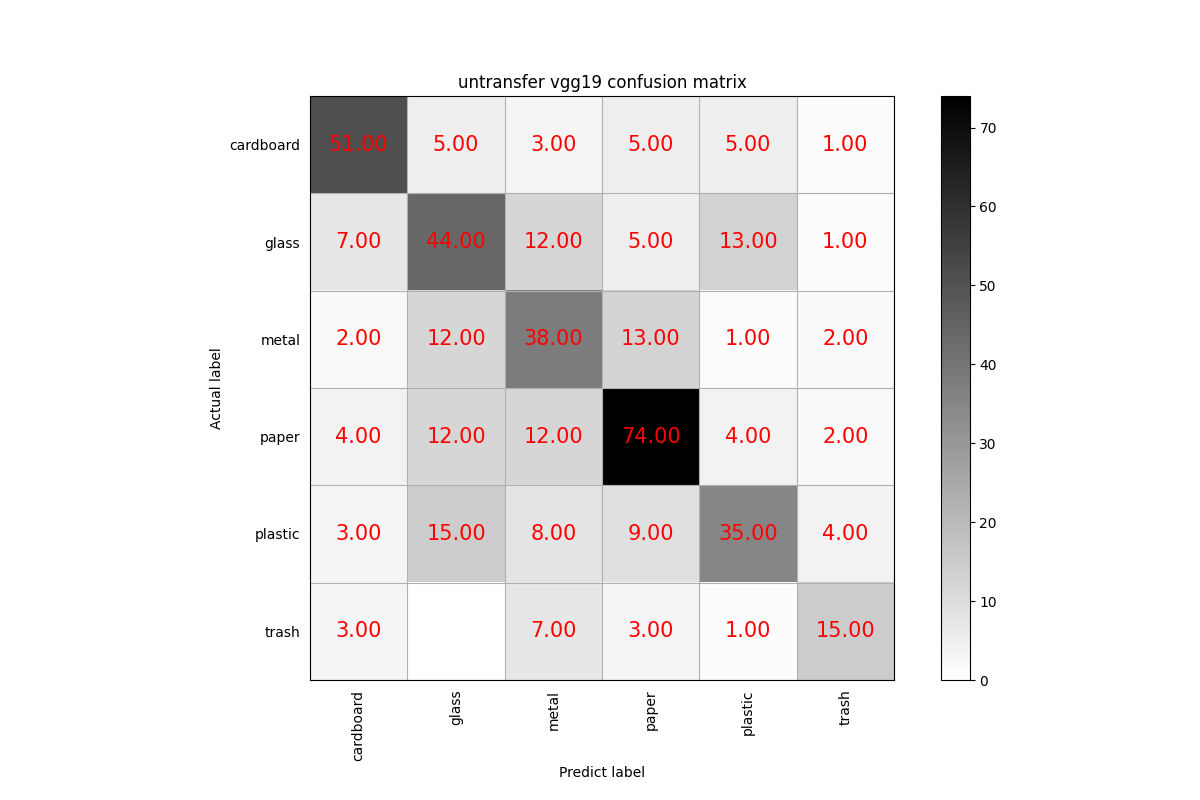
\includegraphics[scale=0.5]{cm/unvgg19.png} 
\subsubsection{ResNet18}
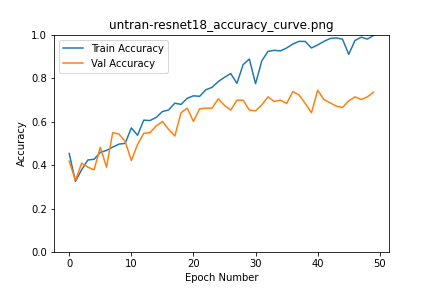
\includegraphics[scale=0.5]{image/untran-resnet18_accuracy_curve.png} 
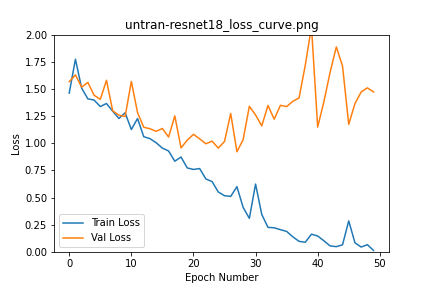
\includegraphics[scale=0.5]{image/untran-resnet18_loss_curve.png} 

测试集上的结果:

\begin{tabular}{|c|c|c|c|c|c|c|}
\hline 
类别 & Cardboard & Glass & Metal & Paper & Plastic & Trash \\ 
\hline 
Accuracy &0.9512761 & 0.89559165& 0.90719258& 0.9187935 & 0.90023202& 0.95359629\\
 \hline 
Recall &0.88571429 &0.6097561 & 0.66176471& 0.89814815& 0.75675676& 0.65517241\\ 
\hline 
Precision &0.82666667& 0.79365079& 0.72580645& 0.80165289& 0.69135802& 0.65517241   \\ 
\hline 
F1 Score &0.85517241& 0.68965517 &0.69230769& 0.84716157 &0.72258065& 0.65517241 \\ 
\hline 
\end{tabular}

混淆矩阵:

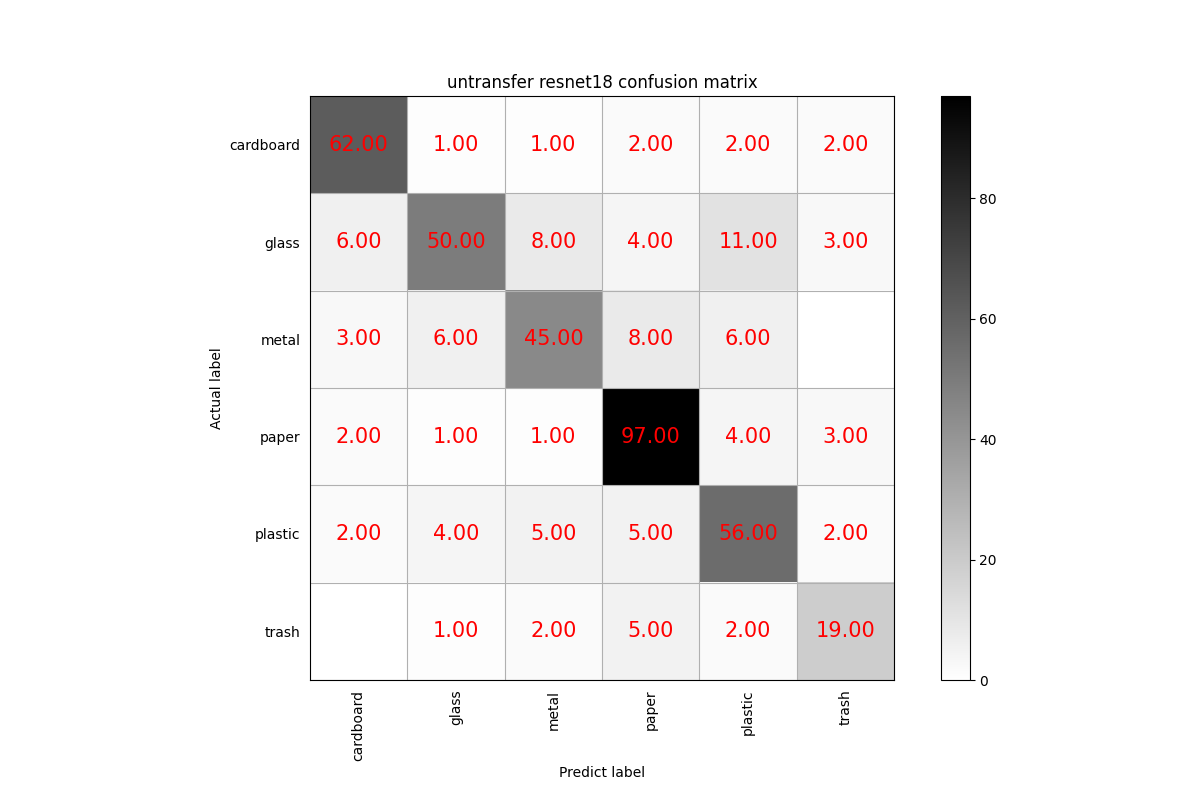
\includegraphics[scale=0.5]{cm/unres18.png} 

\subsubsection{ResNet34}
 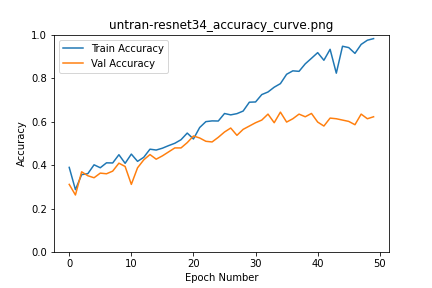
\includegraphics[scale=0.5]{image/untran-resnet34_accuracy_curve.png} 
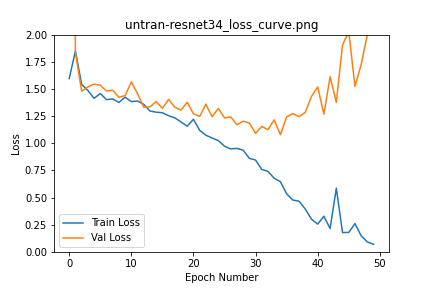
\includegraphics[scale=0.5]{image/untran-resnet34_loss_curve.png} 


测试集上的结果:

\begin{tabular}{|c|c|c|c|c|c|c|}
\hline 
类别 & Cardboard & Glass & Metal & Paper & Plastic & Trash \\ 
\hline 
Accuracy &0.92575406& 0.83294664 &0.83990719& 0.84222738& 0.83990719& 0.91647332\\
 \hline 
Recall &0.7    &    0.51219512& 0.52941176& 0.67592593& 0.66216216 &0.31034483\\ 
\hline 
Precision &0.81666667& 0.56756757 &0.49315068& 0.68867925& 0.52688172& 0.36  \\ 
\hline 
F1 Score &0.75384615& 0.53846154& 0.5106383 & 0.68224299& 0.58682635& 0.33333333 \\ 
\hline 
\end{tabular}

混淆矩阵:

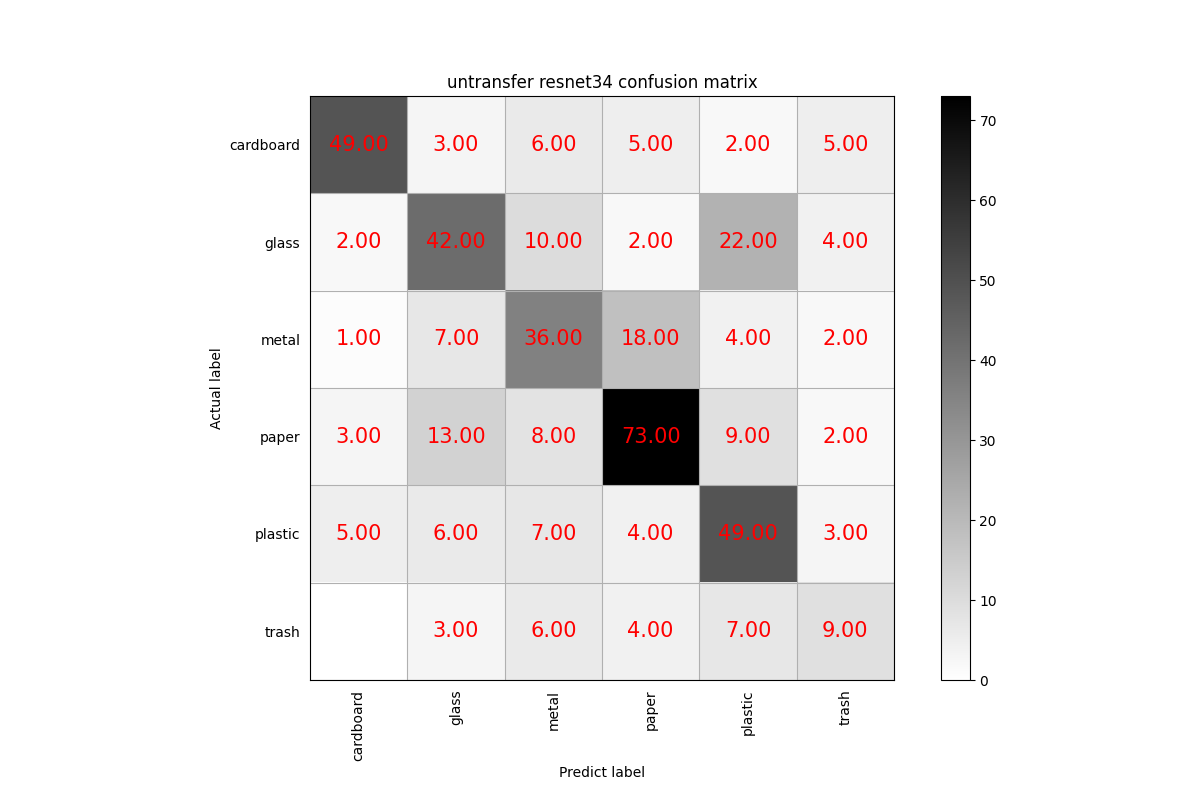
\includegraphics[scale=0.5]{cm/unresnet34.png} 

\subsubsection{ResNet50}
 
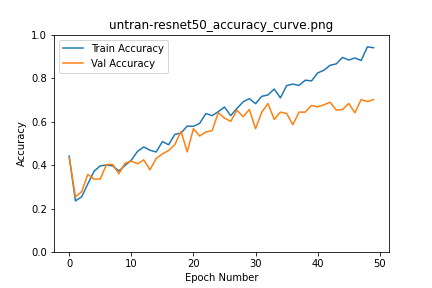
\includegraphics[scale=0.5]{image/untran-resnet50_accuracy_curve.png} 
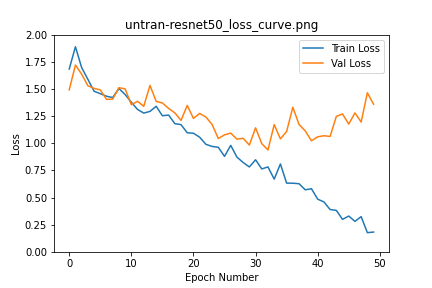
\includegraphics[scale=0.5]{image/untran-resnet50_loss_curve.png} 

测试集上的结果:

\begin{tabular}{|c|c|c|c|c|c|c|}
\hline 
类别 & Cardboard & Glass & Metal & Paper & Plastic & Trash \\ 
\hline 
Accuracy &0.9675174 & 0.95591647& 0.95823666& 0.9350348 & 0.95591647& 0.97215777\\
 \hline 
Recall &0.9       & 0.90243902& 0.94117647& 0.85185185& 0.86486486& 0.65517241\\ 
\hline 
Precision &0.9       & 0.87058824& 0.82051282& 0.88461538& 0.87671233& 0.9047619\\ 
\hline 
F1 Score &0.9       & 0.88622754& 0.87671233& 0.86792453& 0.8707483 & 0.76 \\ 
\hline 
\end{tabular}

混淆矩阵:
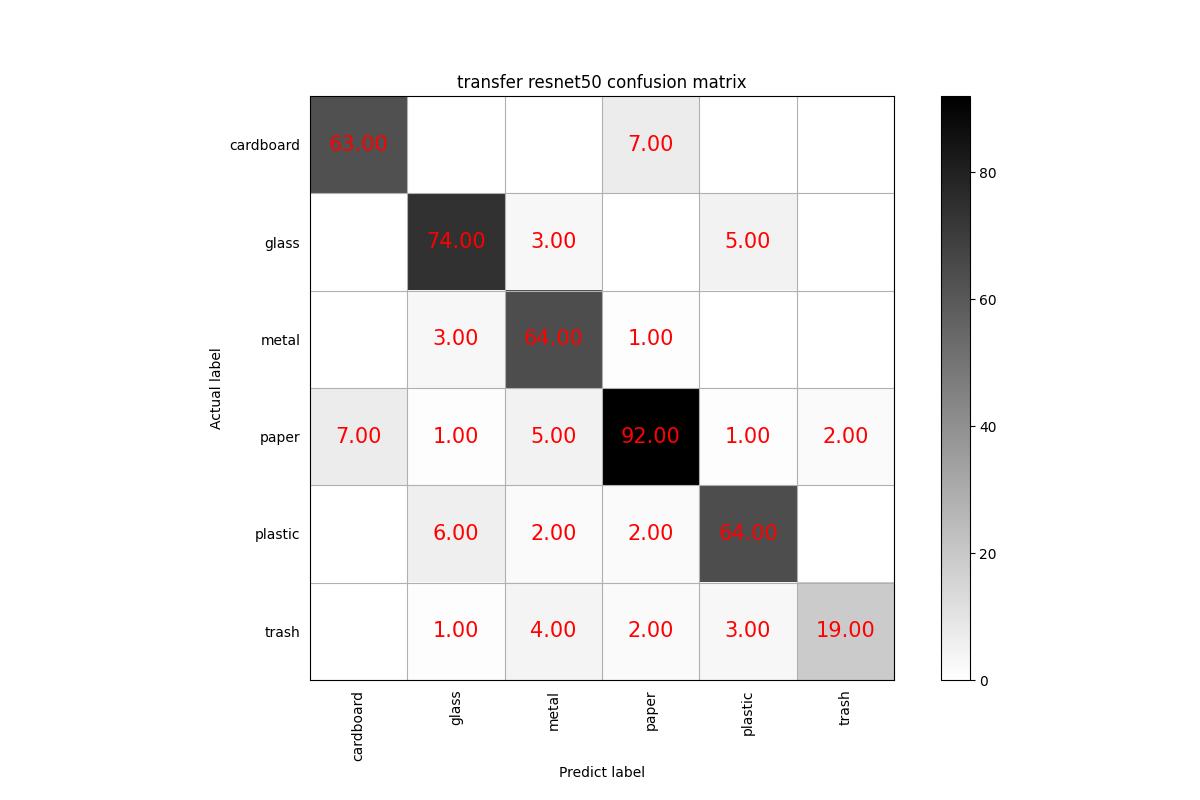
\includegraphics[scale=0.5]{cm/res50.png} 

\subsubsection{ResNet101}
 
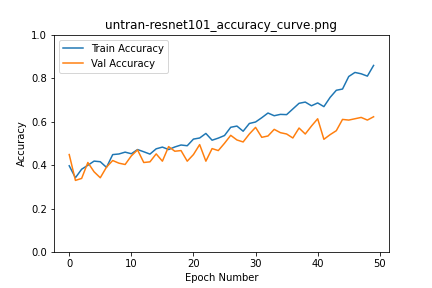
\includegraphics[scale=0.5]{image/untran-resnet101_accuracy_curve.png} 
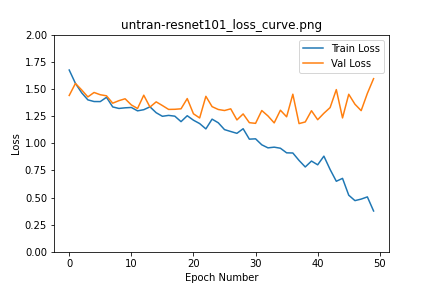
\includegraphics[scale=0.5]{image/untran-resnet101_loss_curve.png}

\begin{tabular}{|c|c|c|c|c|c|c|}
\hline 
类别 & Cardboard & Glass & Metal & Paper & Plastic & Trash \\ 
\hline 
Accuracy &0.94431555& 0.87935035 &0.87935035& 0.90951276& 0.86542923& 0.92807425\\
 \hline 
Recall &0.74285714& 0.6097561&  0.67647059& 0.80555556& 0.72972973& 0.48275862\\ 
\hline 
Precision &0.89655172& 0.71428571 &0.60526316& 0.82857143& 0.58695652& 0.46666667\\ 
\hline 
F1 Score &0.8125&     0.65789474 &0.63888889& 0.81690141& 0.65060241& 0.47457627 \\ 
\hline 
\end{tabular}



测试集上的结果:


混淆矩阵:

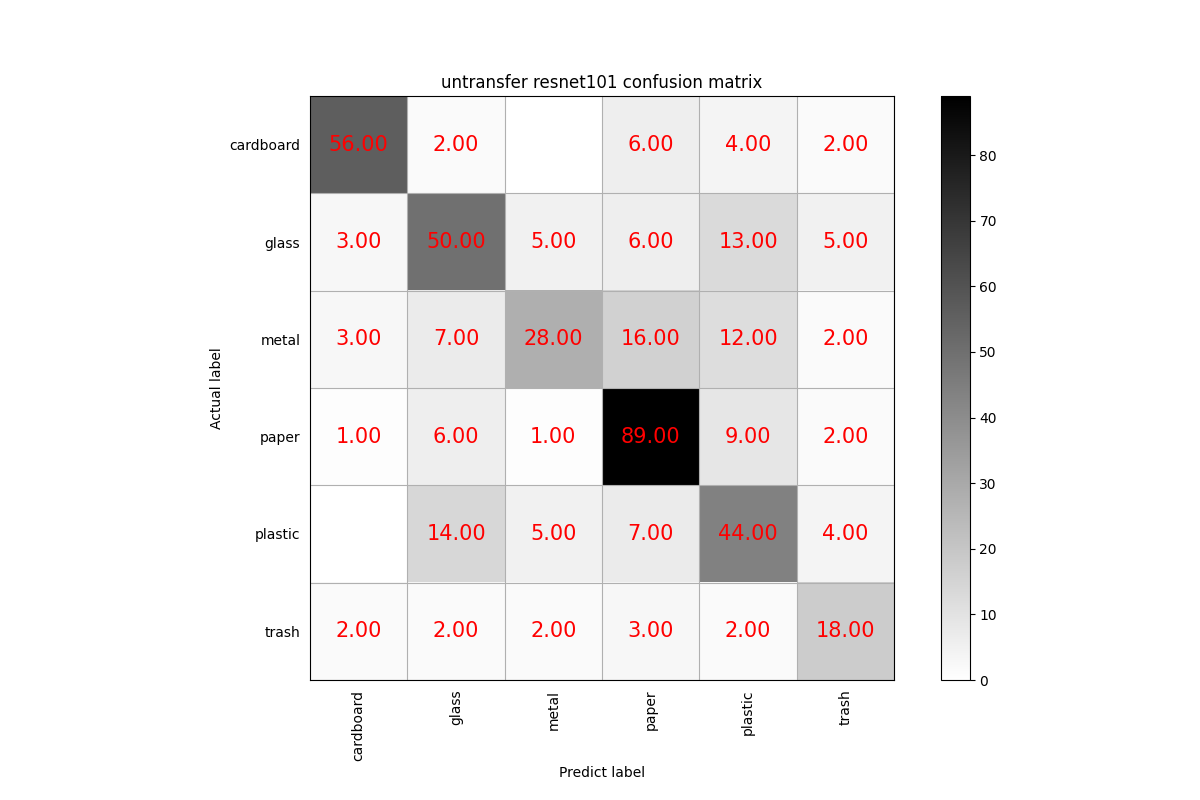
\includegraphics[scale=0.5]{cm/unres101.png} 

\subsubsection{MobileNet\_V2}

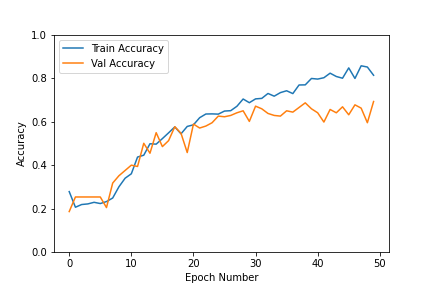
\includegraphics[scale=0.5]{image/mobilenet_v2_36_ADAM_accuracy_curve.png} 
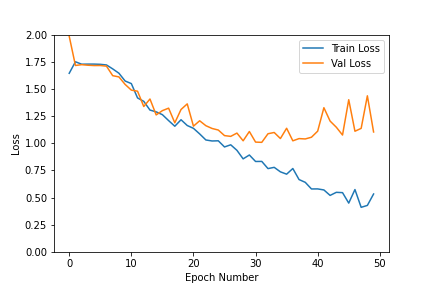
\includegraphics[scale=0.5]{image/mobilenet_v2_36_ADAM_loss_curve.png} 

测试集上的结果:

\begin{tabular}{|c|c|c|c|c|c|c|}
\hline 
类别 & Cardboard & Glass & Metal & Paper & Plastic & Trash \\ 
\hline 
Accuracy &0.92111369& 0.76798144 &0.85382831& 0.86774942& 0.85150812& 0.9350348\\
 \hline 
Recall &00.74285714& 0.54878049& 0.33823529& 0.72222222 &0.60810811& 0.51724138\\ 
\hline 
Precision &0.76470588& 0.41666667& 0.56097561& 0.74285714 &0.5625    & 0.51724138\\ 
\hline 
F1 Score &0.75362319& 0.47368421 &0.42201835& 0.73239437 &0.58441558& 0.51724138\\ 
\hline 
\end{tabular}

混淆矩阵:

 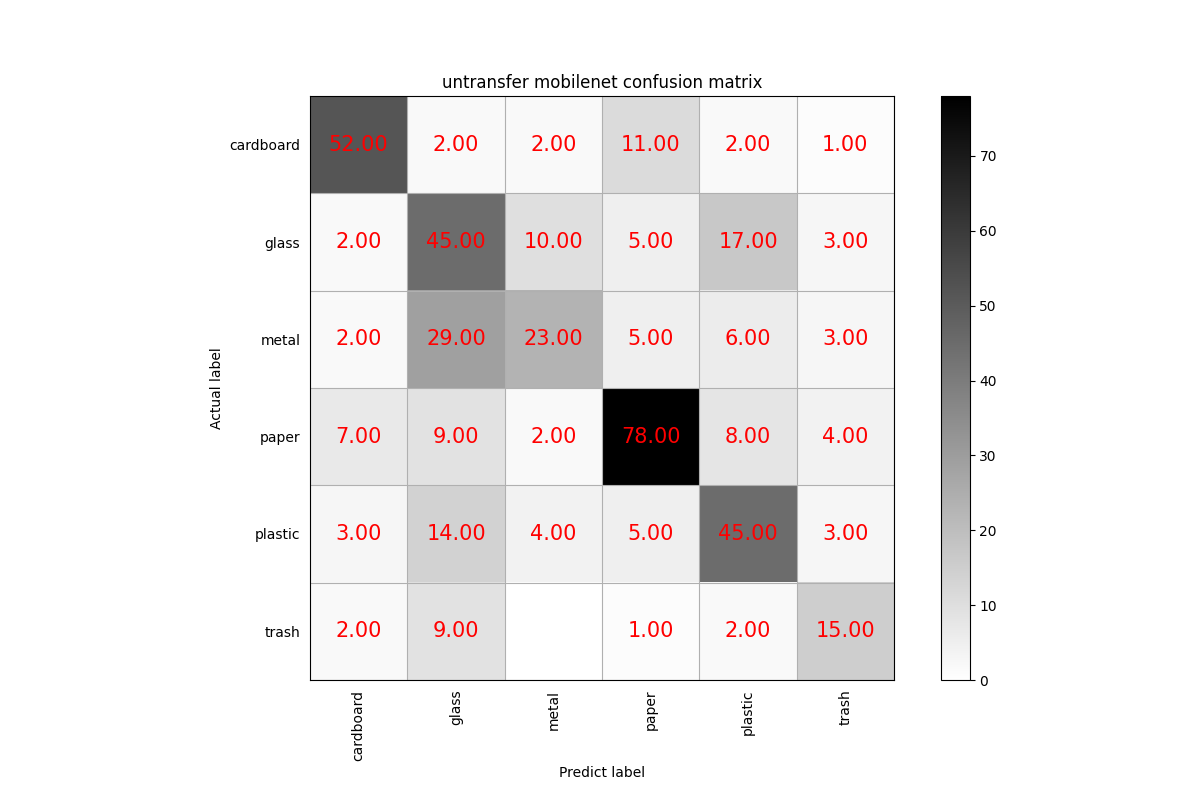
\includegraphics[scale=0.5]{cm/untranmobile.png} 
\subsubsection{DenseNet121}
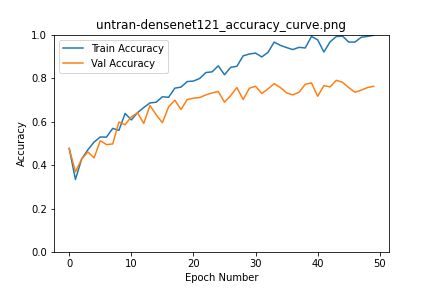
\includegraphics[scale=0.5]{image/untran-densenet121_accuracy_curve.png} 
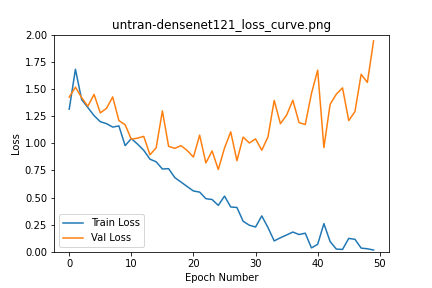
\includegraphics[scale=0.5]{image/untran-densenet121_loss_curve.png} 

测试集上的结果:

\begin{tabular}{|c|c|c|c|c|c|c|}
\hline 
类别 & Cardboard & Glass & Metal & Paper & Plastic & Trash \\ 
\hline 
Accuracy &0.9512761&  0.90487239& 0.91415313& 0.93735499& 0.91183295& 0.96287703\\
 \hline 
Recall &0.84285714& 0.7804878 & 0.91176471& 0.86111111& 0.59459459& 0.65517241\\ 
\hline 
Precision &0.85507246& 0.73563218 &0.66666667& 0.88571429& 0.84615385& 0.76 \\ 
\hline 
F1 Score &0.84892086 &0.75739645 &0.77018634& 0.87323944& 0.6984127 & 0.7037037\\ 
\hline 
\end{tabular}

混淆矩阵:

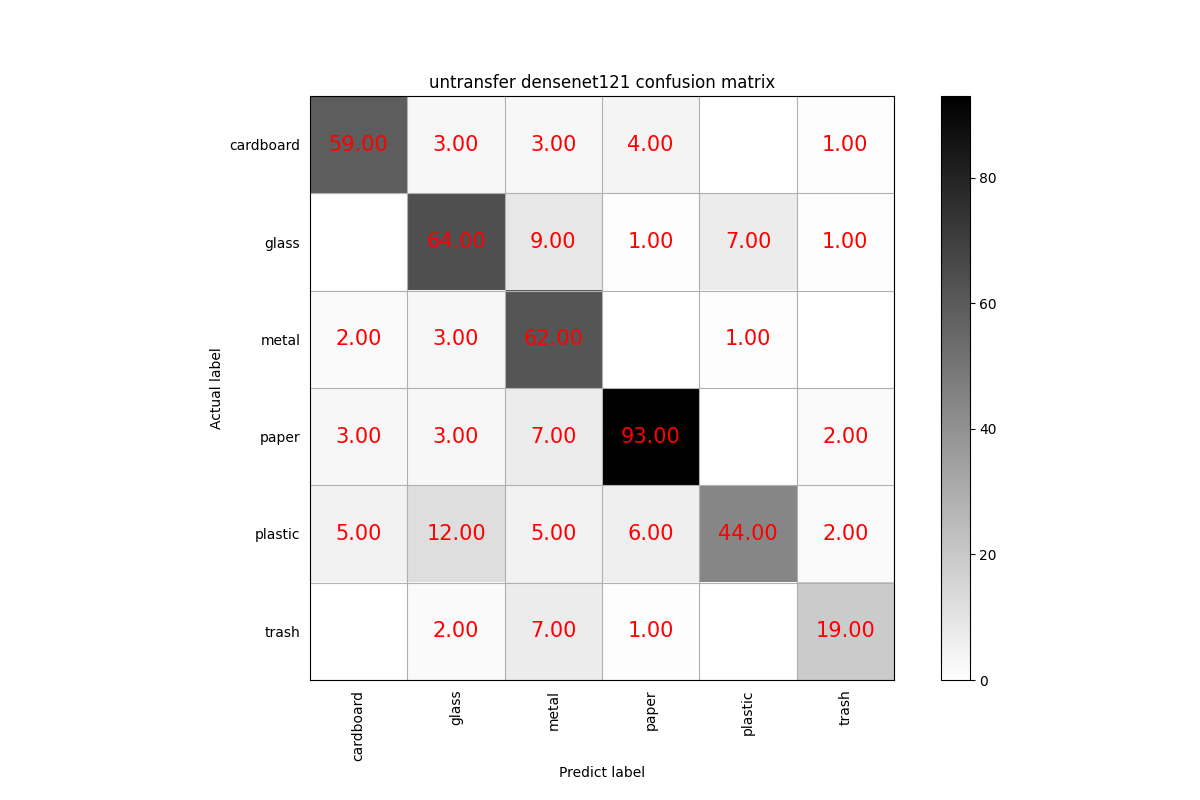
\includegraphics[scale=0.5]{cm/undense121.png} 

\subsubsection{DenseNet161}

测试集上的结果:

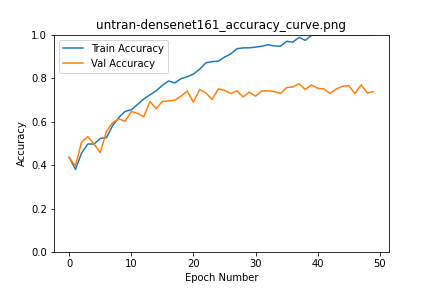
\includegraphics[scale=0.5]{image/untran-densenet161_accuracy_curve.png} 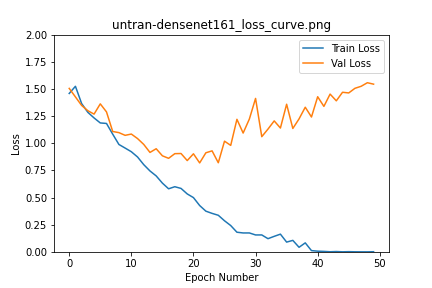
\includegraphics[scale=0.5]{image/untran-densenet161_loss_curve.png} 

\begin{tabular}{|c|c|c|c|c|c|c|}
\hline 
类别 & Cardboard & Glass & Metal & Paper & Plastic & Trash \\ 
\hline 
Accuracy &0.95823666 &0.92343387& 0.92575406& 0.93039443 &0.90719258& 0.96519722\\
 \hline 
Recall &0.82857143 &0.74390244& 0.80882353 &0.89814815& 0.75675676 &0.68965517\\ 
\hline 
Precision &0.90625   & 0.83561644& 0.74324324& 0.8362069 & 0.71794872& 0.76923077\\ 
\hline 
F1 Score &0.86567164& 0.78709677& 0.77464789& 0.86607143 &0.73684211& 0.72727273\\ 
\hline 
\end{tabular}

混淆矩阵:

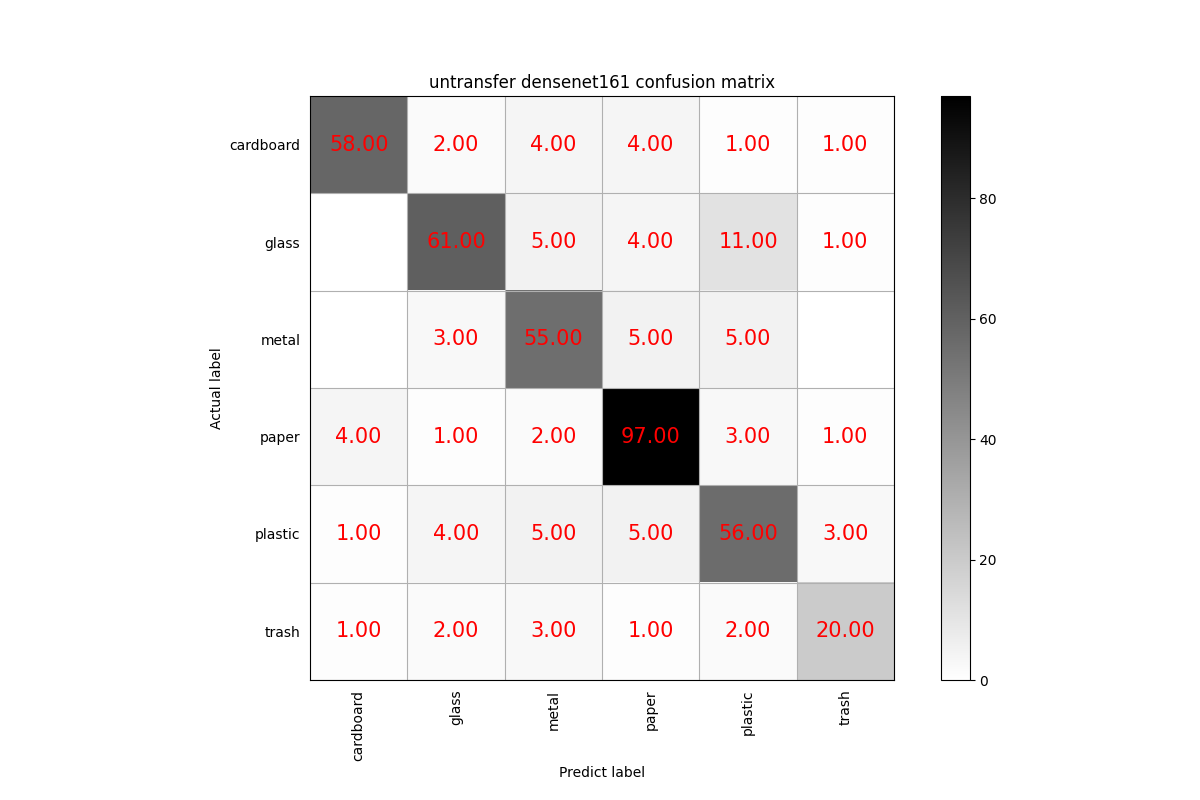
\includegraphics[scale=0.5]{cm/undense161.png} 

\subsection{进行迁移学习(加载了云训练参数)的神经网络训练结果}
\subsubsection{AlexNet}
 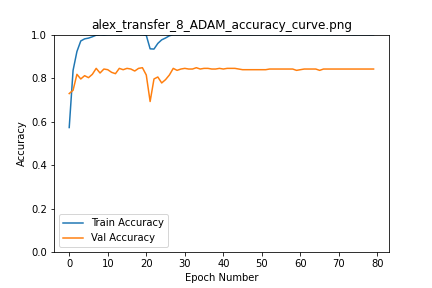
\includegraphics[scale=0.5]{image/alex_transfer_8_ADAM_accuracy_curve.png} 
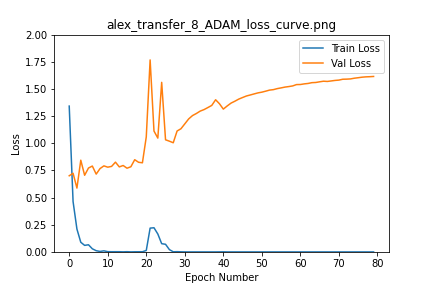
\includegraphics[scale=0.5]{image/alex_transfer_8_ADAM_loss_curve.png} 


在测试集上的训练结果

\begin{tabular}{|c|c|c|c|c|c|c|}
\hline 
类别 & Cardboard & Glass & Metal & Paper & Plastic & Trash \\ 
\hline 
Accuracy &0.9675174 & 0.90023202 &0.9350348 & 0.95823666& 0.91183295& 0.97447796 \\
 \hline 
Recall &0.85714286& 0.73170732 &0.76470588& 0.91666667 &0.83783784& 0.75862069 \\ 
\hline 
Precision &0.9375    & 0.74074074& 0.8125    & 0.91666667& 0.70454545& 0.84615385 \\ 
\hline 
F1 Score &0.89552239& 0.73619632 &0.78787879& 0.91666667& 0.7654321 & 0.8 \\ 
\hline 
\end{tabular} 

混淆矩阵:

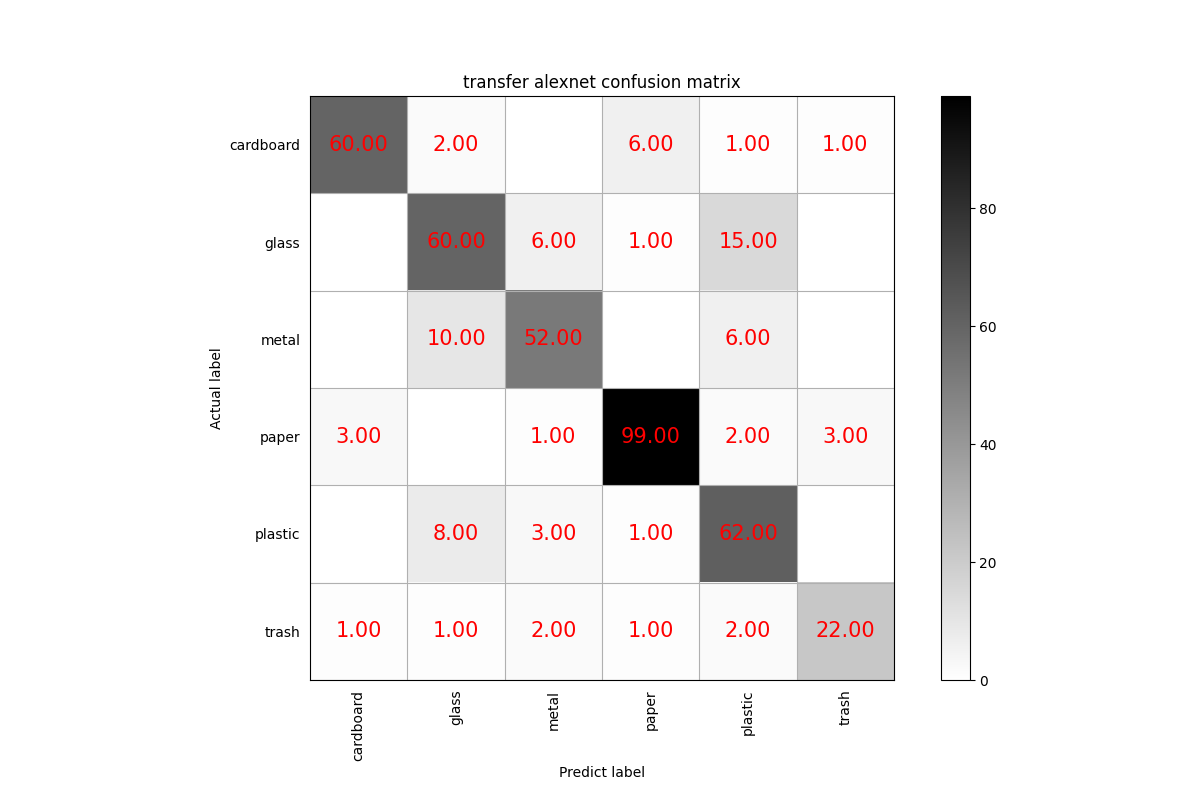
\includegraphics[scale=0.5]{cm/alexnet.png} 

\subsubsection{VGG16\_bn}
 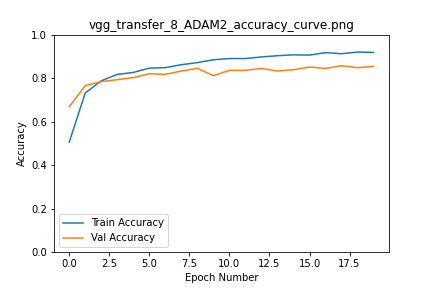
\includegraphics[scale=0.5]{image/vgg_transfer_8_ADAM2_accuracy_curve.png} 
 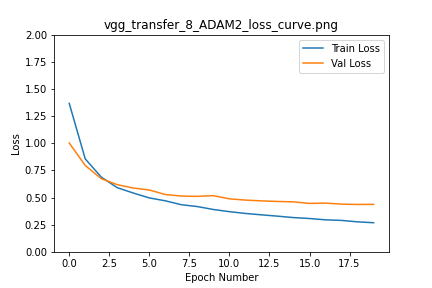
\includegraphics[scale=0.5]{image/vgg_transfer_8_ADAM2_loss_curve.png} 



测试集上的结果:

\begin{tabular}{|c|c|c|c|c|c|c|}
\hline 
类别 & Cardboard & Glass & Metal & Paper & Plastic & Trash \\ 
\hline 
Accuracy &0.97679814& 0.94663573& 0.97215777& 0.94895592& 0.94431555& 0.97911833\\
 \hline 
Recall &0.88571429& 0.87804878 &0.92647059& 0.92592593& 0.82432432& 0.79310345\\ 
\hline 
Precision &00.96875   & 0.84705882 &0.9       & 0.87719298& 0.84722222& 0.88461538 \\ 
\hline 
F1 Score &0.92537313& 0.86227545 &0.91304348& 0.9009009&  0.83561644& 0.83636364 \\ 
\hline 
\end{tabular}

混淆矩阵:

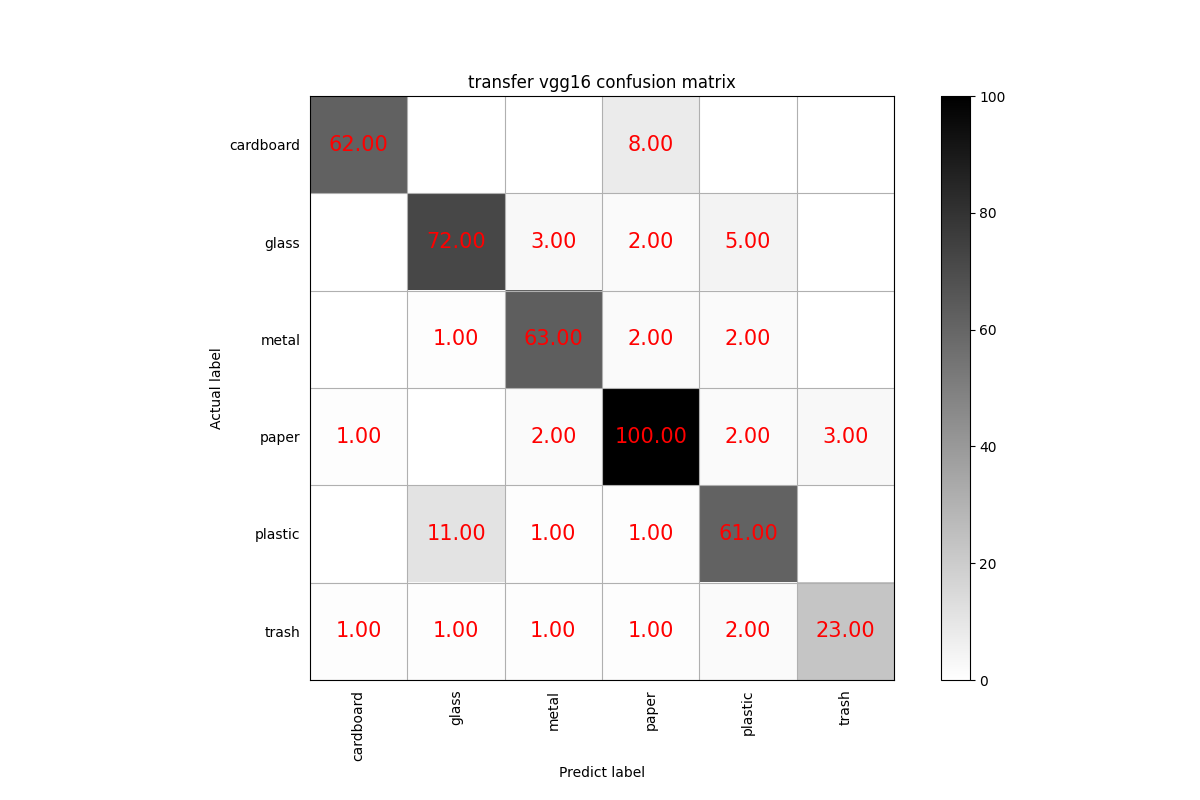
\includegraphics[scale=0.5]{cm/vgg16.png} /

 
\subsubsection{VGG19\_bn}

 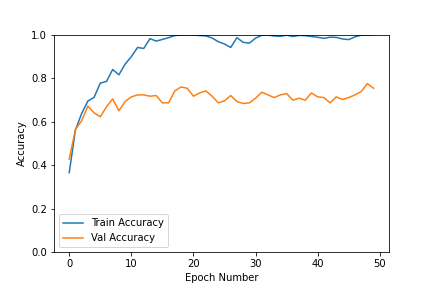
\includegraphics[scale=0.5]{image/vgg19_bn_36_ADAM_accuracy_curve.png} 
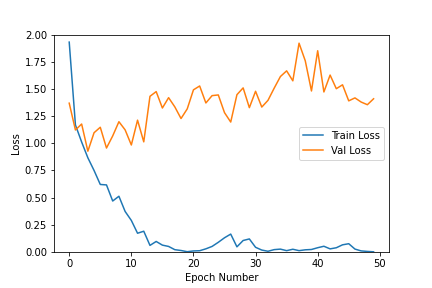
\includegraphics[scale=0.5]{image/vgg19_bn_36_ADAM_loss_curve.png} 

测试集上的训练结果

\begin{tabular}{|c|c|c|c|c|c|c|}
\hline 
类别 & Cardboard & Glass & Metal & Paper & Plastic & Trash \\ 
\hline 
Accuracy &0.97447796& 0.9350348&  0.94431555& 0.95591647& 0.92575406& 0.97679814\\
 \hline 
Recall &0.9       & 0.85365854& 0.79411765& 0.94444444& 0.78378378& 0.75862069\\ 
\hline 
Precision &0.94029851& 0.81395349 &0.84375   & 0.88695652& 0.78378378& 0.88       \\ 
\hline 
F1 Score &0.91970803& 0.83333333 &0.81818182& 0.91479821& 0.78378378& 0.81481481 \\ 
\hline 
\end{tabular}

混淆矩阵:

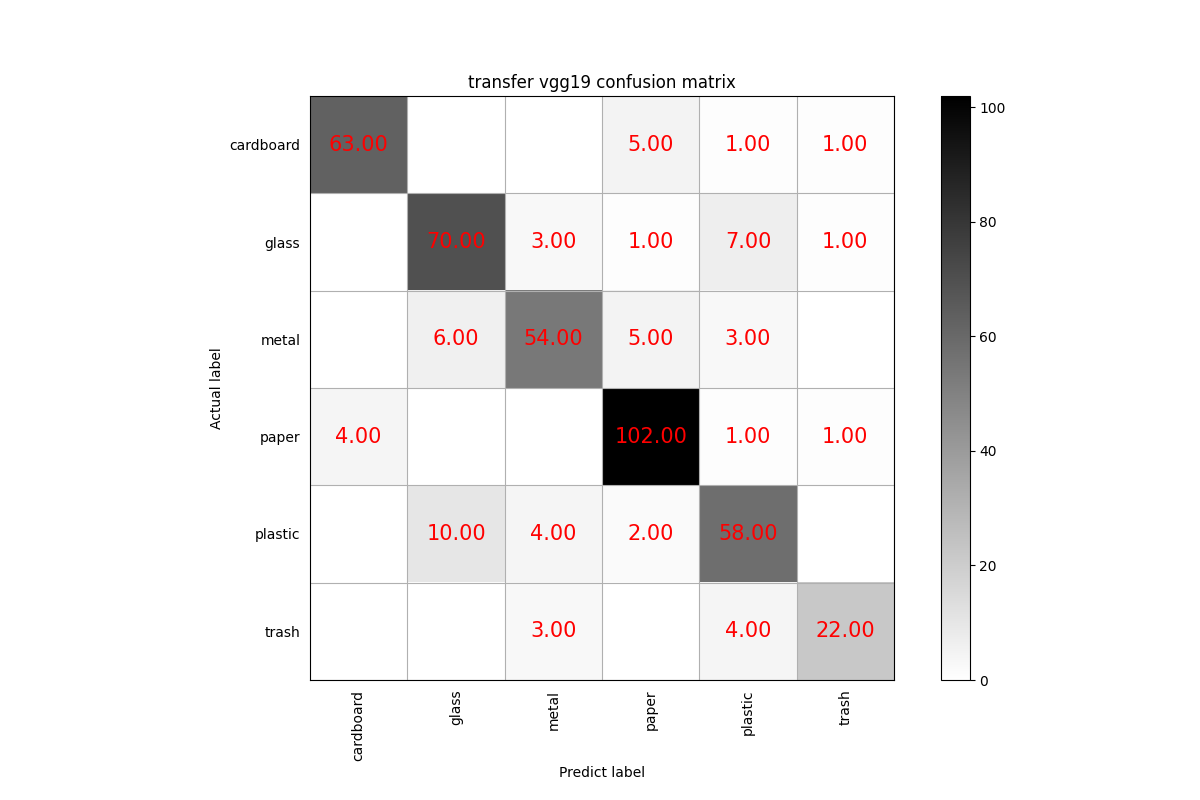
\includegraphics[scale=0.5]{cm/vgg19.png} /

\subsubsection{ResNet18}
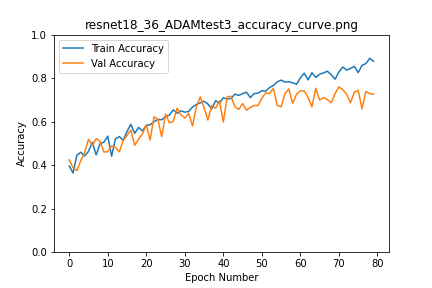
\includegraphics[scale=0.5]{image/resnet18_36_ADAMtest3_accuracy_curve.png} 
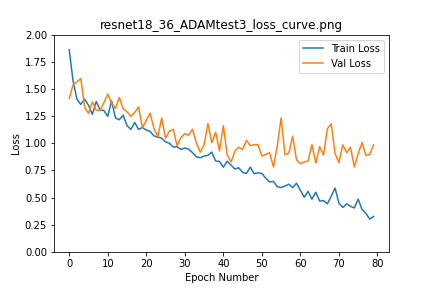
\includegraphics[scale=0.5]{image/resnet18_36_ADAMtest3_loss_curve.png} 

测试集上的结果:

\begin{tabular}{|c|c|c|c|c|c|c|}
\hline 
类别 & Cardboard & Glass & Metal & Paper & Plastic & Trash \\ 
\hline 
Accuracy &0.96983759& 0.93039443 &0.94199536& 0.93735499 &0.93271462& 0.97215777\\
 \hline 
Recall &0.9       & 0.80487805& 0.94117647& 0.84259259& 0.7972973 & 0.68965517\\ 
\hline 
Precision &0.91304348& 0.825  &    0.75294118& 0.9009901 & 0.80821918& 0.86956522   \\ 
\hline 
F1 Score &0.90647482& 0.81481481& 0.83660131& 0.8708134 & 0.80272109& 0.76923077\\ 
\hline 
\end{tabular}

混淆矩阵:

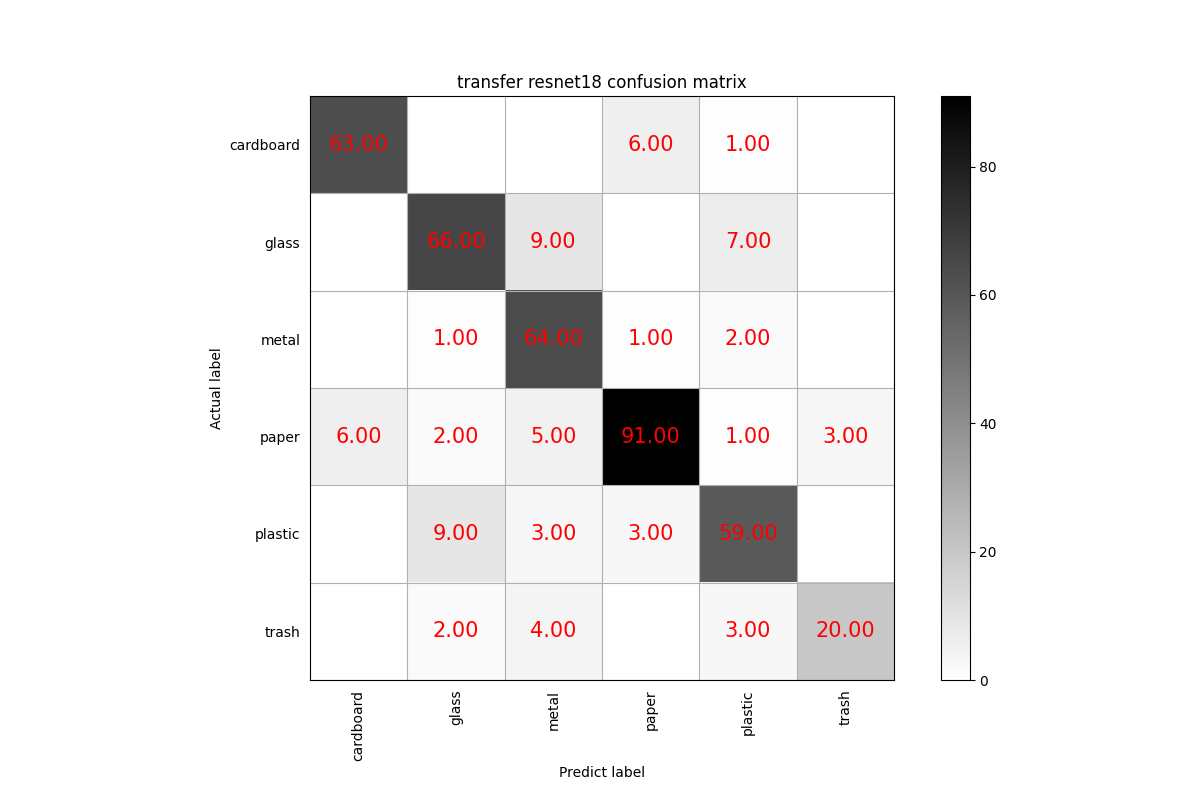
\includegraphics[scale=0.5]{cm/res18.png} 

\subsubsection{ResNet34}
 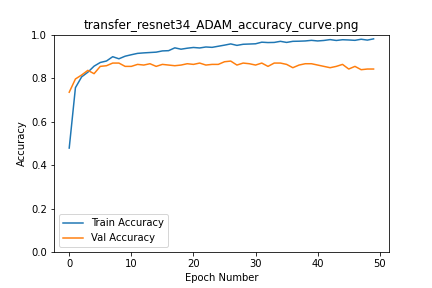
\includegraphics[scale=0.5]{image/transfer_resnet34_ADAM_accuracy_curve.png} 
\includegraphics[scale=0.5]{image/transfer_resnet34_ADAM_loss_curve.png} 


测试集上的结果:

\begin{tabular}{|c|c|c|c|c|c|c|}
\hline 
类别 & Cardboard & Glass & Metal & Paper & Plastic & Trash \\ 
\hline 
Accuracy &0.95823666& 0.92343387& 0.92575406& 0.93039443& 0.90719258& 0.96519722\\
 \hline 
Recall &0.82857143& 0.74390244& 0.80882353& 0.89814815& 0.75675676& 0.68965517\\ 
\hline 
Precision &0.90625   & 0.83561644 &0.74324324& 0.8362069 & 0.71794872& 0.76923077  \\ 
\hline 
F1 Score &0.86567164& 0.78709677& 0.77464789& 0.86607143& 0.73684211& 0.72727273 \\ 
\hline 
\end{tabular}



\subsubsection{ResNet50}
 
\includegraphics[scale=0.5]{image/transfer_resnet50_ADAM_accuracy_curve.png} 
\includegraphics[scale=0.5]{image/transfer_resnet50_ADAM_loss_curve.png} 

测试集上的结果:

\begin{tabular}{|c|c|c|c|c|c|c|}
\hline 
类别 & Cardboard & Glass & Metal & Paper & Plastic & Trash \\ 
\hline 
Accuracy &0.97911833& 0.95359629& 0.96983759& 0.95359629& 0.92343387& 0.96519722\\
 \hline 
Recall &0.91428571& 0.84146341 &0.91176471& 0.90740741 &0.87837838& 0.62068966\\ 
\hline 
Precision &0.95522388& 0.90789474& 0.89855072& 0.90740741& 0.73033708& 0.81818182\\ 
\hline 
F1 Score &0.93430657& 0.87341772& 0.905109497& 0.90740741 &0.79754601& 0.70588235\\ 
\hline 
\end{tabular}

混淆矩阵:

\includegraphics[scale=0.5]{cm/res50.png} 

\subsubsection{ResNet101}
 
\includegraphics[scale=0.5]{image/transfer_resnet101_ADAM_accuracy_curve.png} 
\includegraphics[scale=0.5]{image/transfer_resnet101_ADAM_loss_curve.png} 

测试集上的结果:

\begin{tabular}{|c|c|c|c|c|c|c|}
\hline 
类别 & Cardboard & Glass & Metal & Paper & Plastic & Trash \\ 
\hline 
Accuracy &0.94663573 &0.85382831 &0.87703016& 0.86774942& 0.83758701& 0.93967517\\
 \hline 
Recall &0.8      &  0.6097561 & 0.41176471& 0.82407407& 0.59459459& 0.62068966\\ 
\hline 
Precision &0.86153846& 0.61728395& 0.68292683& 0.7007874 & 0.52380952& 0.54545455\\ 
\hline 
F1 Score &0.82962963 &0.61349693 &0.51376147& 0.75744681& 0.55696203& 0.58064516\\ 
\hline 
\end{tabular}

混淆矩阵:

\includegraphics[scale=0.5]{cm/res101.png} 

\subsubsection{MobileNet\_V2}
\includegraphics[scale=0.5]{image/transfer_mobilenet_ADAM_accuracy_curve.png} 
\includegraphics[scale=0.5]{image/transfer_mobilenet_ADAM_loss_curve.png} 
 

测试集上的结果:

\begin{tabular}{|c|c|c|c|c|c|c|}
\hline 
类别 & Cardboard & Glass & Metal & Paper & Plastic & Trash \\ 
\hline 
Accuracy &0.97447796& 0.94199536& 0.9675174 & 0.9512761  &0.92575406& 0.97911833\\
 \hline 
Recall &0.87142857 &0.86585366& 0.89705882& 0.91666667& 0.82432432& 0.75862069\\ 
\hline 
Precision &0.96825397& 0.83529412& 0.89705882 &0.89189189 &0.7625    & 0.91666667\\ 
\hline 
F1 Score &0.91729323& 0.8502994 & 0.89705882 &0.90410959& 0.79220779& 0.83018868\\ 
\hline 
\end{tabular}

混淆矩阵:

\includegraphics[scale=0.5]{cm/mobile.png}

\subsubsection{DenseNet121}
 
\includegraphics[scale=0.5]{image/transfer_Densenet121_Adam_accuracy_curve.png} 
\includegraphics[scale=0.5]{image/transfer_Densenet121_Adam_loss_curve.png} 



测试集上的结果:

\begin{tabular}{|c|c|c|c|c|c|c|}
\hline 
类别 & Cardboard & Glass & Metal & Paper & Plastic & Trash \\ 
\hline 
Accuracy &0.9675174 & 0.94663573& 0.94431555& 0.95359629& 0.94199536& 0.95823666\\
 \hline 
Recall &0.88571429 &0.90243902& 0.82352941& 0.90740741 &0.82432432& 0.62068966\\ 
\hline 
Precision &0.91176471& 0.83146067& 0.82352941& 0.90740741& 0.83561644& 0.72   \\ 
\hline 
F1 Score &0.89855072 &0.86549708& 0.82352941& 0.90740741& 0.82993197& 0.66666667\\ 
\hline 
\end{tabular}

混淆矩阵:

\includegraphics[scale=0.5]{cm/dense121.png} 

\subsubsection{DenseNet161}

测试集上的结果:

\includegraphics[scale=0.5]{image/transfer_Densenet161_Adam_accuracy_curve.png} 
\includegraphics[scale=0.5]{image/transfer_Densenet161_Adam_loss_curve.png} 


\begin{tabular}{|c|c|c|c|c|c|c|}
\hline 
类别 & Cardboard & Glass & Metal & Paper & Plastic & Trash \\ 
\hline 
Accuracy &0.9837587&  0.96055684& 0.96055684& 0.96287703 &0.95591647& 0.97679814\\
 \hline 
Recall &0.92857143& 0.90243902& 0.89705882& 0.94444444& 0.87837838& 0.72413793\\ 
\hline 
Precision &0.97014925& 0.89156627& 0.85915493& 0.91071429& 0.86666667& 0.91304348\\ 
\hline 
F1 Score &0.94890511& 0.8969697 & 0.87769784& 0.92727273& 0.87248322& 0.80769231\\ 
\hline 
\end{tabular}

\includegraphics[scale=0.5]{cm/dense161.png} port/cm/

\subsection{不同优化方法下的对比}
\subsubsection{Adam VS SGD VS RMSprop}

\includegraphics[scale=0.5]{image/efficient-net_8_ADAM_accuracy_curve.png} 
\includegraphics[scale=0.5]{image/efficient-net_8_ADAM_loss_curve.png}

\includegraphics[scale=0.5]{image/efficient-net_8_RMSprop_accuracy_curve.png} 
\includegraphics[scale=0.5]{image/efficient-net_8_RMSprop_loss_curve.png} 

\includegraphics[scale=0.5]{image/efficient-net_8_SGD_accuracy_curve.png} 
\includegraphics[scale=0.5]{image/efficient-net_8_SGD_loss_curve.png}

Adam数据

\begin{tabular}{|c|c|c|c|c|c|c|}
\hline 
类别 & Cardboard & Glass & Metal & Paper & Plastic & Trash \\ 
\hline 
Accuracy &0.98 &0.99& 0.99& 0.97& 0.98 &0.99\\
 \hline 
Recall &0.91& 0.95& 0.99& 0.96& 0.95 &0.97\\ 
\hline 
Precision &0.97& 0.97& 0.97& 0.94& 0.93 &0.93\\ 
\hline 
F1 Score &0.94& 0.96& 0.98& 0.95& 0.94& 0.95\\ 
\hline 
\end{tabular}

RMSprop数据

\begin{tabular}{|c|c|c|c|c|c|c|}
\hline 
类别 & Cardboard & Glass & Metal & Paper & Plastic & Trash \\ 
\hline 
Accuracy &0.99& 0.97& 0.96 &0.98 &0.97 &0.98\\
 \hline 
Recall &0.94 &0.93& 0.93& 0.95& 0.89 &0.9\\ 
\hline 
Precision &0.99 &0.93& 0.85& 0.96& 0.93 &0.87\\ 
\hline 
F1 Score &0.96 &0.93& 0.89& 0.96 &0.91& 0.88\\ 
\hline 
\end{tabular}

SGD数据

\begin{tabular}{|c|c|c|c|c|c|c|}
\hline 
类别 & Cardboard & Glass & Metal & Paper & Plastic & Trash \\ 
\hline 
Accuracy &0.99 &0.97& 0.98 &0.98& 0.97& 0.98\\
 \hline 
Recall &0.94& 0.91& 0.93 &0.97& 0.93 &0.79\\ 
\hline 
Precision &0.97& 0.93& 0.94& 0.94 &0.88& 0.92\\ 
\hline 
F1 Score &0.96& 0.92& 0.93& 0.95 &0.91& 0.85\\ 
\hline 
\end{tabular}

\includegraphics[scale=0.5]{cm/efficient_net_Adam.png} 

\includegraphics[scale=0.5]{cm/efficient_net_RMSprop.png} 

\includegraphics[scale=0.5]{cm/efficient_net_SGD.png} 

\subsection{模型性能对比}
训练硬件:RTX2080TI
Batchsize:36 EfficientNet batchsize是12

\begin{tabular}{|c|c|c|}
\hline 
模型种类 & 模型文件大小(MB) & 训练时间(每个epoch) \\ 
\hline 
AlexNet & 165 & 9.40 \\ 
\hline 
VGG16 & 537 &  10.984\\ 
\hline 
VGG19 & 558 & 12.376 \\ 
\hline 
MobileNet & 9.12 & 8.6232 \\ 
\hline 
ResNet18 & 44.8&8.1402  \\ 
\hline 
ResNet34 & 85.3 & •9.7024\\ 
\hline 
ResNet50& 94.3 & 10.497 \\ 
\hline 
ResNet101 & 171 & 18.81 \\ 
\hline 
DenseNet121& 28.3 & 8.47\\ 
\hline 
DenseNet161 & 107 & 11.747 \\ 
\hline 
EfficientNet\_B7(RMSProp) & 257 & 195.79\\ 
\hline
EfficientNet\_B7(Adam) & 257 & 165.29\\ 
EfficientNet\_B7(SGD) & 257 & 170.13\\ 
\hline
\end{tabular} 

\section{总结}
\subsection{迁移学习与普通监督学习的对比}
\begin{itemize}
\item 迁移学习模型更容易收敛模型没有发生过拟合的现象 
\item 直接加载模型容易发生过拟合的现象
\item 迁移模型在验证集上的表现更好,在测试集上也展现的较高的准确度
\end{itemize}

\subsection{几种模型的对比}
\begin{itemize}
\item Efficient Net 得到了最好的训练结果 在各个分类上的准确率能够达到92以上,召回率F1的score等表现都非常好
\item MobileNet 展现了非常好的便携性和训练速度 它在精度和性能上面做到了最好的平衡
\end{itemize}
\subsection{模型层数与BN的使用}
\begin{itemize}
\item ResNet分别测试了18、34、50、101四种模型 发现精度并不是随着模型的深度的增加而增加,50与101的表现区别不大
而对于DenseNet  161的表现比较出色但是训练时间较长
\item 实验中有测试vgg16 与vgg16\_bn 两种模型 带了BatchNormalization的模型收敛的更快,同时最后的准确度较好。
\end{itemize}
\subsection{几种训练方式的对比}
\begin{itemize}
\item 在训练EfficientNet的时候发现SGD最后得到的结果非常好就是时间耗费有点多
\item RMSprop中间发生了非常多的动荡最后发生了过拟合
\item Adam算法它比较兼顾时间和性能
\end{itemize}
\section{讨论与展望}
未来可以在模型结构上进行修改从而达到更加好的结果。

可以压缩模型参数改善训练速度和储存空间的问题

对于过拟合的现象找到较合适的解决方案。

\end{document}